\chapter{Аналитический раздел}
\section{Категоризация эмоциональных данных}
Одной из главных проблем в исследованиях, связанных с определением эмоционального состояния диктора по голосу, является отсутствие четкого определения эмоции. Подход к классификации эмоций влияет на процесс аннотирования. Сегодня широко используются три подхода к категоризации эмоциональных данных: дискретный, многомерный и гибридный.
\subsection{Дискретное пространство эмоций}
Дискретный подход основан на выделении фундаментальных (базовых) эмоций, сочетания которых порождают разнообразие эмоциональных явлений. Разные авторы называют разное число таких эмоций~--~от двух до десяти. П.~Экман на основе изучения лицевой экспрессии выделяет пять базовых эмоций: гнев, страх, отвращение, печаль и радость. Первоначальная версия 1999 года также включала удивление. \cite{Ekman1972, Ekman1992} Р.~Плутчик \cite{Plutchik1980} выделяет восемь базисных эмоций, деля их на четыре пары, каждая из которых связана с определенным действием: страх, уныние, удивление и т.~д. 

На сегодняшний день существование базовых эмоций ставится под сомнение. Теория встречает ряд концептуальных проблем, таких как, например, эмпирическое определение набора базовых эмоций или критерии синхронизации эмоциональных реакций. Однако, многие решения в области автоматического детектирования эмоций основаны на дискретной модели эмоциональной сферы. Например, решение компании <<Affectiva>>.~\cite{Affectica}

\subsection{Многомерное пространство эмоций}
Многомерное пространство представляет собой эмоции в координатном многомерном пространстве. В качестве ее источника рассматривают идею В. Вундта о том, что многогранность чувств
человека можно описать с помощью трех измерений: удовольствие-неудовольствие, расслабление-напряжение, возбуждение-успокоение. Вундт заключил, \cite{Вундт1984} что эти измерения охватывают все разнообразие эмоциональных состояний. Данные для этой теории были получены с помощью метода интроспекции.

Эмоциональная сфера представляется как многомерное пространство, образованное некоторым
количеством осей координат. Оси задаются полюсами первичных характеристик эмоций. Отдельные эмоции~--~это точки, местоположение которых в <<эмоциональном>> пространстве определяется степенью выраженности этих параметров.

Один из примеров описываемого подхода~--~модель Дж.~Рассела. В ней водится двумерный базис, в котором каждая эмоция характеризуется валентностью (\textit{англ. valence}) и интенсивностью (\textit{англ. arousal}). Измерение валентности отражает то,
насколько хорошо человек ощущает себя на уровне субъективного переживания от максимального неудовольствия до максимального удовольствия. Измерение активации связано с
субъективным чувством энергии и ранжируется в диапазоне от дремоты до бурного возбуждения. Такой подход используется, например, в наборе данных <<RECOLA>> \cite{RECOLA}.

Аналогично вопросу о количестве эмоций в дискретной модели, вопрос о количестве измерений остается открытым. Использование только двух критикуется на том основании, что они не позволяют устанавливать различия между отдельными эмоциональными состояниями (например, страх, гнев, ревность, презрение и др. имеют отрицательную валентность и высокую активацию).

\subsection{Гибридное пространство эмоций}
Гибридная модель представляет собой комбинацию дискретной и многомерной модели. Примером такой модели являются <<Песочные часы эмоций>>, предложенные Камбрией, Ливингстоном и Хуссейном.~\cite{hourglass} 

Согласно этой классификации, в отдельной области $n$-мерного эмоционального пространства различия между эмоциями могут определяться в терминах измерений, имеющих отношение к этой области. Эмоции могут быть сопоставимы по измерениям внутри и вне категорий, и каждая категория может иметь свои отличительные признаки.~\cite{Russell2003} Каждое измерение характеризуется шестью уровнями силы, с которой выражены эмоции. Данные уровни обозначаются набором из двадцати четырех эмоций. Поэтому совершенно любая эмоция может рассматриваться как и фиксированное состояние, так и часть пространства, связанная с другими эмоциями нелинейными отношениями. 

\section{Наборы данных речевых эмоций}
\subsection{Наборы данных на иностранных языках}
\textbf{Набор данных RAVDESS.} \cite{ravdess} Набор содержит записи 24 профессиональных актеров (12 мужчин и 12 женщин), озвучивающих две одинаковые фразы на английском языке с североамериканским акцентом в двух вариантах: речь и пение. На каждого актера набор предоставляет 60 записей. Использовано дискретное эмоциональное пространство, состоящее из семи эмоций: спокойствие, гнев, страх, отвращение и радость. Каждая фраза представлена двумя уровнями эмоциональной интенсивности для каждой из эмоций и безэмоционально. 

\textbf{Набор данных  SAVEE} \cite{savee} \textit{(англ. Surrey Audio-Visual Expressed Emotion)} состоит из
речи четырех актеров мужского пола, говорящих на английском с британским акцентом. Эмоциональные типы для каждого высказывания соответствуют одной из шести базовых эмоций (радость, печаль, гнев, удивление, страх, отвращение) или нейтральному состоянию. Всего было записано 15 уникальных фраз, каждая фраза записывалась безэмоционально дважды.

\textbf{Набор данных Emo-DB.} \cite{emodb} Немецкие актеры (5 женщин и 5 мужчин) имитировали эмоции, произнося фразы, интонационно отражающие различные эмоции (гнев, радость, печаль, страх), а также произнести некоторые из них так, чтобы они не несли никакой эмоциональной нагрузки. Смысл фраз не соответствовал интонационному оформлению. Запись файлов для базы данных проводилась в звукоизолированной комнате. Для оценки качества записанной речи в Берлинском университете был проведен перцептивный тест которым было предложено оценить, к какой из эмоций относится прослушанная единожды запись. Сообщения с уровнем распознавания выше 80\% и естественностью звучания свыше 60\% вошли в итоговый набор.

\textbf{Набор данных  TESS} \cite{tess} \textit{(англ. Toronto emotional speech set)} содержит 2800 звуковых дорожек формата <<WAV>>. Набор озвучен только женскими голосами и размечен по 6 базовым эмоциям: гнев, отвращение, страх, счастье, печаль, удивление. Также присутствуют записи безэмоциональной речи.
\subsection{Наборы данных на русском языке}
\textbf{Набор данных RUSLANA}. \cite{ruslana} Является первым рускоязычным эмоциональным набором данных. Содержит записи 61 человека (12 мужчин и 49 женщин), которые произносили десять предложений с выражением следующих эмоциональных состояний: удивление, счастье, гнев, грусть и страх. Также предложения были записаны безэмоционально. Таким образом, в сумме база содержит 3 660 записей. Общая продолжительность аудиозаписей составляет более 31 часа. 

\textbf{Набор данных DUSHA} \cite{dusha} -- русскоязычный набор эмоциональных данных. Состоит из нарезки русскоязычных подкастов, содержащие до пяти слов. Все аудиозаписи были сделаны на профессиональные микрофоны. Разметка осуществлялась также согласно дискретной модели и содержала следующие эмоции: радость, грусть, злость. Также присутствуют безэмоциональные записи. Набор содержит примерно из 300 000 аудиозаписей, суммарная длительность которых около 350 часов. В разметке содержится 1,5 млн записей. 

\textbf{Русскоязычный эмоциональный корпус (REC)} \cite{rec} состоит из 295 видеозаписей университетских зачетов и экзаменов и 510 видеозаписей общения с клиентами в службе одного окна ГУ ИС г. Москвы. К настоящему моменту размечено 192 файла. Разметка содержит информацию о мимике и жестах, которая размещена на временной шкале. Учитывается мимика двух органов: глаза (взгляды вверх и по сторонам продолжительностью больше 0,5-1 с) и рот (неречевые движения губ, манипуляции языком и движения челюстью). Движения рук представлены как самостоятельные, так и с использованием сторонних предметов, тела или одежды.

\subsection{Сравнение существующих эмоциональных корпусов}
Сравнение существующих корпусов представлен в таблице \ref{tab:class}. 
\begin{table}[H]
	\centering
	\caption{Сравнение существующих эмоциональных корпусов}\label{tab:class}
	\resizebox{\textwidth}{!}{
		\begin{tabular}{|c|c|c|c|c|c|}
			\hline
			\textit{Название} & \textit{Количество эмоций} & \multicolumn{2}{c|}{\textit{Количество голосов}} & \textit{Лексикон} & \textit{Есть в открытом} \\ \cline{3-4}
			\textit{корпуса} & \textit{в разметке} & \textit{мужских} & \textit{женских} & \textit{} & \textit{доступе} \\ \hline
			RAVDESS & 7 & 12 & 12 & 2 предл. & да \\ \hline
			SAVEE & 6 & 4 & 0 & 15 предл. & да \\ \hline
			Emo-DB & 6 & 5 & 5 & 10  предл. & да \\ \hline
			TESS & 7 & 0 & 2 & 200 слов & да \\ \hline
			RUSLANA & 4 & 12 & 49 & 10  предл. & нет \\ \hline
			DUSHA (crowd) & 4 & - & - & обширный & да \\ \hline
			DUSHA (podcast) & 4 & - & - & обширный & да \\ \hline
			REC & - & - & - & обширный & нет \\ \hline
		\end{tabular}
	}
\end{table}
Прочерк в графе <<Количество голосов>> означает, что практически для каждой записи в корпусе голос уникальный. Прочерк в графе <<Количество эмоций в разметке>> означает отсутствие эмоциональной разметки.

Существующие корпуса имеет смысл сравнивать, во-первых, по размеру представленных данных. При увеличении размера корпуса улучшается статистическая значимость результатов, что позволяет получать более точные оценки параметров модели. На данный момент самым большим русскоязычным набором данных является DUSHA. 

Также следует обратить внимание на разнообразие корпуса, а именно на количество представленных голосов. Разнообразие обучающего корпуса может существенно влиять на точность классификации. Если корпус содержит небольшое количество голосов, то модель может не обладать достаточной обобщающей способностью и не сможет правильно классифицировать новые данные. Однако, стоит учитывать, что классификатор может потерять способность обобщения и перестать обнаруживать закономерности в данных при перегрузке эмоциональными классами. В большинстве представленных корпусов за основу взята <<большая шестерка>> эмоций П.~Экмана \cite{Ekman1972}. Теория шести базовых эмоций в настоящее время хоть и ставится под сомнение, для аффективных вчислений такой подход является наиболее эффективным, поскольку при расширении эмоционального пространства эмоции могут быть слабо различимы. 

Также на качество классификации может влиять качество самих аудиофайлов, поскольку информативные признаки, характеризующие эмоцию (например, частота основного тона или превых формант) могут быть чувствительны к шуму или искажениям в записи. Поэтому для корпусов, использующихся в распознавании эмоций из звучащей речи, запись аудиофайлов желательно производить в студийных условиях.

В большинстве существующих датасетов эмоции симулируются, то есть привлекается небольшая группа профессиональных актеров, озвучивающих заданные фразы. В таком случае далеко не всегда удается отразить реальные эмоциональные состояния человека. Также излишняя театральность при симуляции эмоций может отрицательно повлиять на результат. Однако, симуляция эмоций может быть полезной в тех случаях, когда для получения набора данных с реальными эмоциями участников исследования недостаточно ресурсов.

\subsection{Интонационный контур при выражении эмоций}
Звучащие предложения обладают интонацией: повествовательной, вопросительной, ответной, перечислительной, восклицательной и т.п. Предполагается, что существует связь между выражением эмоции и использованием одного из существующих в русском языке интонационного контура. \cite{intonation} В русском языке выделяют 7 интонационных контуров (ИК): \cite{ik}
\begin{itemize}
	\item \textbf{ИК-1} характеризуется понижением тона на ударной части:\\
	\textit{<<Анна стоит на мосту. Наташа поет.>>},\\
	используется для выражения завершенности в повествовательных предложениях;
	\item при \textbf{ИК-2} ударная часть произносится с некоторым повышением тона:\\
	\textit{<<Кто пьет сок? Как поет Наташа?>>},\\
	наблюдается в вопросе с вопросительными словами;
	\item \textbf{ИК-3} характеризуется значительным повышением тона на ударной части:\\
	\textit{<<Это Антон? Ее зовут Наташа?>>},\\
	наблюдается в вопросе без вопросительных слов;
	\item \textbf{ИК-4} характеризуется повышением тона, продолжающееся на безударных слогах:\\
	\textit{<<А вы? А это?>>},\\
	наблюдается в вопросе без вопросительных слов;
	\item \textbf{ИК-5} используется при выражении оценки в предложениях с местоименными словами:\\
	\textit{<<Какой сегодня день!>>},\\
	наблюдается повышение тона на ударной части;
	\item \textbf{ИК-6}, аналогично ИК5, используется при выражении оценки в предложениях с местоименными словами, однако повышение тона происходит на ударной части и продолжается на заударной части:\\
	\textit{<<Какой сок вкусный!>>};
	\item \textbf{ИК-7}, аналогично ИК-1 используется для выражения завершенности в повествовательных предложениях:\\
	\textit{<<И Антон стоит на мосту.>>},\\
	но ударная часть, в отличие от ИК-1, эмоционально окрашена.
\end{itemize}
ИК в сочетании с некоторыми артикуляционными особенностями может выступать в качестве средства выражения эмоций. Однако, не каждая эмоция может быть выражена с использованием всех семи ИК. Например, эмоция удивления выражается с помощью ИК-2, ИК-3, ИК-4 и ИК-6. \cite{conn} Такая связь важна для систем распознавания эмоций в речи. Результат работы классификатора -- набор вероятностей принадлежности высказывания к тому или иному эмоциональному классу. Если вероятности принадлежности высказывания к нескольким эмоциональным классам схожа по значению, то решение принимается на основе дополнительной информации о высказывании. В качестве дополнительной информации имеет смысл использовать номер интонационного контура. На данный момент ни один корпус эмоциональной речи не содержит информацию об ИК.

\section{Выделение информативных признаков}
Важной особенностью речевого сигнала является его условная стационарность на небольших промежутках (от 20 до 40 мс).~\cite{frames} По этой причине для оцифровки сигнал разделяется на фреймы. Деление происходит таким образом, чтобы каждая точка перекрывалась дважды.~\cite{mfcc-steps}

Задача распознавания эмоций решается непосредственно по оцифрованному сигналу. Выделяется два этапа решения задачи: выделение и отбор информативных признаков и классификация (сопоставление признаков).


Даже при работе с фреймами, сигнал содержит много избыточной для анализа информации. Поэтому для того, чтобы привести сигнал в вид, который будет использован алгоритмом распознавания, требуется выделить набор информативных признаков речевого сигнала. К выделяемому набору признаков предъявляются следующие требования: \cite{features-must}
\begin{itemize}
	\item с помощью выделенного набора признаков можно получить наиболее значимую информацию из акустического сигнала;
	\item размер выборки должен быть минимальным для увеличения быстродействия разрабатываемой системы распознавания эмоций.
\end{itemize}
Характеристики речевого сигнала, использующиеся для определения эмоций по речи, можно разделить на две группы: просодические и спекртальные. 

Просодическими признаками, содержащими информацию об эмоции, являются характеристики, основанные на количественной оценке ЧОТ, интенсивность (энергия) речевого сигнала, темп речи и паузация. К спектральным признакам можно отнести различные кепстральные (например, мел-кепстральные) коэффициенты, частоты первых формант речевого сигнала и их среднеквадратические отклонения, энергетические (джиттер и шиммер) и пертурбационные параметры.

\subsection{Просодические характеристики}
\subsubsection{Частота основного тона}
Значение частоты основного тона зависит от размеров и степени натяжения связок. \cite{acoustics-tone} Кроме самой частоты основного тона оценивается ее среднеквадратическое отклонение. В таблице \ref{tab:pinch} представлена связь между эмоцией и изменением этих характеристик относительно безэмоциональной речи.
\begin{table}[H]
	\centering
	\caption{Связь характеристик частоты основного тона и эмоции}
	\begin{tabular}{|T|TT|}
		\hline
		\multirow{2}{*}{\textit{Базовая эмоция}} & \multicolumn{2}{>{\centering\arraybackslash}p{0.6\textwidth}|}{\textit{Изменение значений относительно нейтрального состояния}} \\ \cline{2-3} 
		& \multicolumn{1}{T|}{\textit{ЧОТ}} & \textit{СКО ЧОТ} \\ \hline
		Радость & \multicolumn{1}{T|}{выше} & выше \\ \hline
		Печаль & \multicolumn{1}{T|}{ниже} & ниже \\ \hline
		Гнев & \multicolumn{1}{T|}{ниже} & выше \\ \hline
		Удивление & \multicolumn{1}{T|}{ниже} & выше \\ \hline
		Страх & \multicolumn{1}{T|}{выше} & выше \\ \hline
	\end{tabular}
	\label{tab:pinch}
\end{table}

Методы определения частоты основного тона можно разделить на три категории: основанные на временной динамике сигнала (\textit{англ. time-domain}), основанные на частотной структуре (\textit{англ. frequency-domain}) и комбинированные методы. \cite{pitch}

Перед применением методов, основанных на временной динамике, сигнал предварительно фильтруют, оставляя только низкие частоты. Задаются минимальная и максимальная частоты (например, от 75 до 500 Гц). Частота основного тона не определяется для участков, содержащих негармоничную речь (паузы, шумовые звуки), поскольку это влечет за собой ошибки, которые могут распространяться на соседние фреймы при применении интерполяции или сглаживания. Длину фрейма выбирают так, чтобы в ней содержалось как минимум три периода.

В методах, основанных на частотной структуре, анализируется гармоническая структура сигнала. Одним из таких методов является кепстральный анализ. Кепстр -- результат преобразования, получаемого применением обратного преобразования Фурье к логарифму спектра мощности сигнала. Иными словами, кепстр является спектром от спектра сигнала.

Алгоритм получения кепстра можно разделить на три этапа.
\begin{enumerate}
	\item К сигналу применяется дискретное преобразование Фурье.
	\item От полученного спектра мощности сигнала берется логарифм, чтобы получить лог-спектр.
	\item К лог-спектру применяется обратное преобразование Фурье. На выходе получается спектр от спектра сигнала.
\end{enumerate}

Гибридные методы определения  имеет смысл рассмотреть на примере алгоритма YAAPT (\textit{англ. Yet Another Algorithm of Pitch Tracking}), который считается гибридным, поскольку использует как частотную, так и временную информацию. YAAPT, как и другие алгоритмы определения ЧОТ состоит из трех этапов: препроцессирование, поиск кандидатов (возможных значений ЧОТ) и выбор наиболее вероятной траектории ЧОТ.

На этапе препроцессирования значения изначального сигнала возводят в квадрат для усиления и восстановления пиков автокорреляции. Затем по спектру преобразованного сигнала рассчитывается базовая траектория ЧОТ. Кандидаты определяются с помощью функции SHC~--~\textit{от англ. Spectral Harmonics Correlation} согласно \ref{eq:shc}:

\begin{equation}\label{eq:shc}
	\mathrm{SHC}(t,\,f) = \sum\limits_{f'=-\mathrm{WL}/2}^{\mathrm{WL}/2} \prod\limits_{r=1}^{\mathrm{NH}+1}S(t,\,rf+f'),
\end{equation}
где $S(t,\,f)$ — магнитудный спектр для фрейма $t$ и частоты $f$, $\mathrm{WL}$ — длина окна (Гц), $\mathrm{NH}$~--~число гармоник (рекомендуется \cite{yaapt} использовать первые три гармоники). 

Далее, как для изначального сигнала, так и для преобразованного производится определение кандидатов на F0, и вместо автокорреляционной функции здесь используется функция NCCF~--~\textit{от англ. Normalized Cross Correlation} (\ref{eq:ncff}):

\begin{equation}\label{eq:ncff}
	\mathrm{NCCF}(m) = \frac{\sum\limits_{n=0}^{N-m-1} x(n)\cdot x(n+m)}{\sqrt{\sum\limits_{n=0}^{N-m-1} x^2(n) \cdot \sum\limits_{n=0}^{N-m-1} x^2(n+m)}}\text{,} \hspace{0.3cm} 0 < m < M_{0}
\end{equation}
Далее проводится оценка всех возможных кандидатов и вычисление их веса (\textit{англ. merit}). Вес кандидатов, полученных по аудиосигналу, от амплитуды пика NCCF и от их близости к траектории ЧОТ, определенной по спектру.

Затем для всех пар оставшихся кандидатов рассчитывается матрица цены перехода (\textit{англ. Transition Cost}), по которой находят оптимальную траекторию ЧОТ. 

\subsubsection{Инетнсивность, темп речи и паузация}

Громкость (интенсивность) речи измеряется в децибелах (дБ). Связь градаций интенсивности и эмоции представлена в таблице \ref{tab:inten}.
%	\item шепот: менее 20 дБ;
%	\item значительное снижение: 20$\dots$40 дБ;
%	\item умеренное понижение: 40$\dots$50 дБ;
%	\item нормальная интенсивность: 50$\dots$80 дБ;
%	\item умеренное повышение: 80$\dots$90 дБ;
%	\item значительное повышение: 90$\dots$110 дБ;
%	\item крик: свыше 110 дБ.
%\end{itemize}

\begin{table}[H]
	\centering
	\caption{Связь градаций интенсивности и эмоции}
	\begin{tabular}{|H|H|}
		\hline
		\textit{Интенсивность} & \textit{Значение} (дБ) \\ \hline
		Шепот & < 20 \\ \hline
		Значительное снижение & 20$\dots$40 \\ \hline
		Умеренное снижение & 40$\dots$50 \\ \hline
		Нормальная & 50$\dots$80 \\ \hline
		Умеренное повышение & 80$\dots$90 \\ \hline
		Значительное повышение & 90$\dots$110 \\ \hline
		Крик & > 110 \\ \hline
	\end{tabular}
	\label{tab:inten}
\end{table}


Следующей просодической характеристикой является паузация. Короткими паузами принято считать паузы до 3 секунд, средними -- от 3 до 7 секунд, длинными -- свыше 7 секунд. В таблице \ref{tab:pause} представлена связь характеристик паузации и эмоции.

\begin{table}[H]
	\centering
	\caption{Связь характеристик паузации и эмоции}
	\begin{tabular}{|T|TT|}
		\hline
		\multirow{2}{*}{\textit{Базовая эмоция}} & \multicolumn{2}{>{\centering\arraybackslash}p{0.6\textwidth}|}{\textit{Изменение значений относительно нейтрального состояния}} \\ \cline{2-3} 
		& \multicolumn{1}{T|}{количество пауз} & длина пауз \\ \hline
		Радость & \multicolumn{1}{T|}{меньше} & короче \\ \hline
		Печаль & \multicolumn{1}{T|}{больше} & короче \\ \hline
		Гнев & \multicolumn{1}{T|}{меньше} & короче \\ \hline
		Удивление & \multicolumn{1}{T|}{больше} & длиннее \\ \hline
		Страх & \multicolumn{1}{T|}{больше} & длиннее \\ \hline
	\end{tabular}
	\label{tab:pause}
\end{table}

Темпом речи называют скорость произнесения элементов речи (звуков, слогов, слов). Темп речи изменяется двумя параметрами: \cite{ling-dict}
\begin{itemize}
	\item числом произносимых в единицу времени элементов речи;
	\item средней длительностью элемента.
\end{itemize}
Повышение темпа речи осуществляется за счет сокращения длительности гласных и согласных звуков, снижение темпа достигается путем увеличения длительности гласных. Согласно исследованиям в \cite{emo-vk}, изменение темпа речи связано с проявлением говорящим эмоции. Например, проявление тревожности характеризуется ускорением темпа речи, а холодность и задумчивость -- замедлением.

\subsection{Спектральные характеристики}

\subsubsection{Мел-кепстральные коэффициенты}
%Для представления огибающей спектра, которой описывается форма голосового тракта были введены мел-кепстральные коэффициенты (\textit{англ. MFCC}).~\cite{mfcc}
%Основная идея работы с речью человека
%заключается в том, что звуки, генерируемые человеком, фильтруются формой голосового
%тракта, включая язык, зубы и т. д . Набор этих характеристик и можно представить с помощью
%мел-кепстральных коэффициент ов .
Основной принцип работы с человеческой речью заключается в том, что звуки, генерируемые человеком, фильтруются формой голосового тракта (язык, зубы и т.д.). Набор этих характеристик и можно представить с помощью мел-кепстральных коэффициентов (\textit{англ. MFCC}).~\cite{mfcc}

Шкала Мел (рисунок \ref{fig:mel-hz}) соотносит воспринимаемую частоту или высоту чистого тона (мел) с фактической измеренной частотой (Гц). Люди гораздо лучше различают небольшие изменения высоты звука на низких частотах, чем на высоких.~\cite{mel} 
\begin{figure}[H]
	\centering
	\begin{tikzpicture}
		\begin{axis}[
			legend pos = north west,
			xmin=0, xmax=10000,
			ymin=0, ymax=3200,
			/pgf/number format/.cd,
			use comma,
			1000 sep={},
			xlabel= Фактическая измеренная частота (Гц),
			ylabel= Высота чистого тона (мел) ,
			grid = both,
			grid style = {dashed, lightgray!35},
			xtick distance = 500,
			ytick distance = 200,
			width = 0.98\textwidth,
			tick label style={font=\scriptsize},
			scaled ticks=false,
			height=0.3\textheight,]
			\addplot[
			red,
			semithick,
			domain=-0:10000,
			] {1127.01048 * ln(1 + x /700)};
		\end{axis}
	\end{tikzpicture}
	\caption{График зависимости частоты от мел}
	\label{fig:mel-hz}
\end{figure}

Вычисление мел-кепстральных коэффициентов заключается в следующем. Для каждого фрейма $x_j(n)$ выполняется дискретное преобразование Фурье (\ref{eq:dpf}):
\begin{equation}\label{eq:dpf}
	X_j(k) = \displaystyle\sum_{n = 0}^{N-1} x_j(n)w(n)\exp{-\cfrac{2\pi i}{N}kn},\;0 \leq k < N,
\end{equation}
где $j$~--~номер фрейма, $w(n)$~--~оконная функция Хэмминга, используемая для уменьшения утечки ДПФ на интервале конечной длительности. 

Следующим шагом вычисляется банк мел-фильтров из $M$ треугольных фильтров. Для этого треугольные фильтры умножаются на периодограмму и суммируются. Каждый треугольный фильтр моделируются с помощью функции \ref{eq:mel-filter}:
\begin{equation}\label{eq:mel-filter}
	H_m(k) = \begin{cases}
		0, & k < f(m - 1), \\
		\cfrac{k - f(m - 1)}{f(m) - f(m - 1)}, & f(m - 1) \leq k < f(m),\\
		\cfrac{f(m + 1) - k}{f(m + 1) - f(m)}, & f(m) \leq k < f(m + 1),\\
		0, & k > f(m + 1).\\
	\end{cases}
\end{equation}
Далее производится расчет логарифмического значения энергии компонент спектра на выходе каждого фильтра~(\ref{eq:mel-tmp}):
\begin{equation}\label{eq:mel-tmp}
	T_j(m) = \ln \sum_{k = 0}^{N - 1}P_j(k)H_m(k),\;0 \leq m < M.
\end{equation}
Поскольку ДПФ характеристик синтезированных фильтров \ref{eq:mel-filter} взаимно пересекаются, а энергии на выходе фильтров существенно коррелируют, для вычисления MFCC необходимо использовать дискретное косинусное преобразование (\ref{eq:mel-final}), чтобы устранить возникающие корреляци:
\begin{equation}\label{eq:mel-final}
	c_j(m) = \sum_{m=0}^{M-1}T_j(m)\cos\left(\cfrac{\pi n\left(m + \cfrac{1}{2}\right)}{M}\right),\;0 \leq n < M.
\end{equation}
После получения $c_j(m)$, коэффициент $c_j(0)$ отбрасывается, так как он не несет информации о речи диктора
и задает постоянное смещение.~\cite{frames}

\subsubsection{Энергетические и пертурбационные параметры}

Выделяют следующие энергетические параметры речи: нижний уровень громкости речи ($I_{\mathrm{lower}}$), верхний уровень громкости речи ($I_{\mathrm{higher}}$), динамический диапазон ($\Delta I$) и амплитуда основного тона ($I_{\mathrm{pinch}}$). Энергетические параметры речи измеряются в децибелах (дБ).

Пертурбационными параметрами называют джиттер и шиммер. Существует несколько параметров их оценки. Локальный джиттер определяется согласно \ref{eq:jitter-loc}:
\begin{equation}\label{eq:jitter-loc}
	\mathrm{jitter}_{\mathrm{loc}} = \cfrac{1}{N - 1}\sum_{i = 1}^{N - 1}\left|F_0(i) - F_0(i + 1)\right|\;\bigg/\;
		\cfrac{1}{N}\sum_{N}^{i = 1}F_0(i),
\end{equation}
где $F_0(i)$ -- длительность $i$-го периода основного тона, $N$ -- число периодов основного тона.

Другой способ определения джиттера -- использование отклонения текущей длительности периода не от предыдущей, а от локально усредненного значения, которое рассчитывается на окне в 3 или 5 выборок \cite{farrus2007jitter}:
\begin{equation}\label{eq:jitter}
	\mathrm{jitter}_{\mathrm{P}} = \cfrac{1}{N - P + 1}\sum_{i = 1 + \textstyle\frac{P - 1}{2}}^{N - \textstyle\frac{P - 1}{2}}\;\left|F_0(i) - \cfrac{1}{P}\sum^{i + \textstyle\frac{P - 1}{2}}_{n = i - \textstyle\frac{P - 1}{2}}F_0(n)\right|\bigg/\;\cfrac{1}{N}\sum_{i = 1}^{N}\left|F_0(i)\right|,
\end{equation}
где $P$ -- параметр, определяющий количество периодов используемых для вычисления среднего.


Аналогично джиттеру, для вычисления шиммера существует несколько способов. Простейший -- определение средней абсолютной разницы между амплитудами последовательных периодов основного тона $A(i)$, деленной на среднюю амплитуду (выражение \ref{eq:shimmer-loc}):
\begin{equation}\label{eq:shimmer-loc}
	\mathrm{shimmer}_{\mathrm{loc}} = \cfrac{1}{N - 1}\sum_{i = 1}^{N - 1}\left|A(i) - A(i + 1)\right|\;\bigg/\;
	\cfrac{1}{N}\sum_{N}^{i = 1}A(i).
\end{equation}
Существуют варианты, определения шиммера как относительное отклонение амплитуды от локально-усредненного значения на интервале в $P$ выборок(\ref{eq:shimmer}):
\begin{equation}\label{eq:shimmer}
	\mathrm{shimmer}_{\mathrm{P}} = \cfrac{1}{N - P + 1}\sum_{i = 1 + \textstyle\frac{P - 1}{2}}^{N - \textstyle\frac{P - 1}{2}}\;\left|A(i) - \cfrac{1}{P}\sum^{i + \textstyle\frac{P - 1}{2}}_{n = i - \textstyle\frac{P - 1}{2}}A(n)\right|\bigg/\;\cfrac{1}{N}\sum_{i = 1}^{N}\left|A(i)\right|.
\end{equation}
Такая оценка более точна чем \ref{eq:shimmer-loc}, поскольку на шиммер влияет постепенный равномерный (естественный) спад интенсивности голоса, создающий эффект <<дрейфа>> амплитуды сигнала.~\cite{baken2000clinical} 
\subsubsection{Частоты первых формант речевого сигнала}
Форманты возникают под влиянием резонаторов речевого аппарата, поэтому их высотное положение не зависит от основного тона, но зависит от произносимого звука. При произнесении некоторых звуков речи (в основном гласных) происходит усиление обретонов на определенной частоте: например, при произнесении гласной <<у>> характерно усиление частичных тонов от 200 до 400 Герц, а для гласной <<о>> -- от 400 до 600 Герц.

Определение формант возможно с помощью кепстрального анализа. Речь можно представить как результат свертки инициирующего сигнала гортанных импульсов с частотной характеристикой голосового тракта, выступающего в роли линейного фильтра (\ref{eq:speech}):
\begin{equation}\label{eq:speech}
	x(t) = s(t) * h(t),
\end{equation}
где $s(t)$ - инициирующий сигнал, $h(t)$ -- частотная характеристика голосового тракта. Представляя сигнал во временной области согласно \ref{eq:speech-time}:
\begin{equation}\label{eq:speech-time}
	X(\omega) = S(\omega) \cdot H(\omega),
\end{equation}
при переходе к лог-спектру (\ref{eq:speech-log}) и кепстру (\ref{eq:speech-cepstrum}) можно получить следующие выражения:
\begin{gather}
	\log X(\omega) = \log S(\omega) + \log H(\omega) \label{eq:speech-log}\\
	X(\bar{\omega}) = S(\bar{\omega}) + H(\bar{\omega}) \label{eq:speech-cepstrum}
\end{gather}
То есть свертка сигналов во временной области эквивалентна их умножению в частотной области или сложению в лог-спектре и кепстре. Это свойство кепстра позволяет разделить инициирующий сигнал и частотную характеристику голосового тракта. При этом информация о тембре и формантах будет находиться на низких quefrency-значениях (анаграмма от англ. \textit{frequency}, дословно -- сачтотах) кепстра, а информация о инициирующем сигнале - на высоких.

Чтобы извлечь тот или иной компонент сигнала, нужно применить т.н. liftering (анаграмма от англ. \textit{filtering}, фильтрация) - аналог частотных фильтров для quefrency-области. Для получения информации о формантах можно использовать следующий фильтр низких quefrency-значений:
\begin{equation}
	l(n)
	= 
	\begin{cases}
		1,  n < \tau\\
		-1,  n \ge \tau\\
	\end{cases}
\end{equation}
Для мужской речи значение τ выбирают в диапазоне от 4 до 8 мс, так как среднее значение частоты мужской речи находится в диапазоне от 128 до 270 Гц. Для женской речи, из-за более высокого среднего значения частоты (256-310 Гц), диапазон, на котором расположены форманты в кепстре, может пересекаться с диапазоном инициирующего сигнала, что мешает однозначному разделению компонент речи.

\section{Классификаторы, используемые в анализе речи}
Автоматическое определение эмоций происходит с помощью классификатора -- обученной модели, которая после обучения сможет определять эмоции по записям человеческой речи. Обучение классификатора происходит с использованием одного набора данных на одном языке. Существует множество классификаторов, используемых в схожих с исследуемой задачах -- модель гауссовых смесей, метод опорных векторов, метод k-ближайших соседей. Однако, наиболее популярны при распознавании эмоций модели -- это скрытая марковская модель (\textit{англ. Hidden Markov Model, HMM}) и искусственная нейронная сеть (\textit{англ. Artificial~Neural~Networks, ANN}).

\subsection{Скрытая марковская модель}

Скрытые марковские модели предоставляют более подходящий и более мощный инструмент моделирования в ситуациях когда состояния не являются непосредственно наблюдаемыми. Более детальное объяснение скрытых марковских моделей имеет смысл начать с определения марковских цепей.

Марковская цепь -- это конечный автомат, имеющий дискретное число состояний $q_1, \dots, q_n$ и существует вероятность перехода из состояния $q_i$ в другое состояние $q_j$: $P\left(S_t = q_j | S_{t - 1} = q_i\right)$. Цепь может находиться в состоянии $q_i$ в любой момент времени $t$, поскольку вермя дискретно. Также согласно марковскому свойству, вероятность следующего состояния зависит только от вероятности предыдущего.

Скрытая марковская модель -- это марковская цепь, в которой состояния не являются непосредственно наблюдаемыми. Такую модель можно объяснить как двойной  стохастический процесс: скрытый стохастический процесс, который невозможно наблюдать напрямую и процесс, который создает последовательность наблюдений с учетом первого процесса.

При применении скрытой марковской модели при классификации выделяют три основных задачи. 
\begin{enumerate}
	\item \textit{Задача вычисления оценки}. В рассматриваемой модели необходимо определить оценку вероятности последовательности наблюдений.
	\item \textit{Задача определения оптимальной последовательности}. С учетом модели и конкретной последовательности наблюдений необходимо определить оценку наиболее вероятной последовательности состояний, которая создает эти 	наблюдения.
	\item \textit{Задача обучения параметров}. С учетом количества последовательностей наблюдений необходимо отрегулировать параметры модели.
\end{enumerate}
Для того, чтобы формализовать представленные задачи, следует ввести следующие обозначения. Модель $\lambda = (A,\,B,\,\pi)$ состоит из матрицы перехода $A$, матрицы наблюдаемых значений $B$ и начального распределения $\pi$. Последовательность наблюдаемых значений $D$ выбирается из алфавита (множества значений скрытых параметров) $V$.

Суть первой задачи заключается в определении вероятности последовательности наблюдений $D$ по параметрам данной модели $\lambda = (A,\,B,\,\pi)$. Для вычисления вероятности последовательности наблюдений можно вычислить ее оценку для конкретной последовательности состояний, а затем прибавить вероятности для всех возможных последовательностей состояний согласно \ref{eq:hmm1}:
\begin{equation}\label{eq:hmm1}
	P(D|\lambda) = \sum_{Q}P(D|\,Q,\,\lambda)p(Q|\,\lambda)
\end{equation}

Вторая задача заключается в том, чтобы по модели $\lambda$ и последовательности $D$ найти оптимальную последовательность состояний $Q$. Третья задача -- главная, заключается в оптимизации параметров модели $\lambda = (A,\,B,\,\pi)$ таким образом, чтобы минимизировать $p(D|\lambda)$ при данных $D$, т.е. найти модель максимального правдоподобия. 

\subsection{Искусственная нейронная сеть}
Нейронная сеть -- математическая модель, построенная на принципах функционирования биологических нейросетей (сетей нервных клеток живого организма). \cite{nl} Основная парадигма нейронных сетей -- это формирование решения из множество простых элементов, подобных нейронам. Эти элементы образуют граф с взвешенными синаптическими связями. Искусственная нейронная сеть обладает следующими свойствами: \cite{dukeNL}
\begin{itemize}
	\item параллельность -- в любой момент времени в активном состоянии могут находиться несколько процессов;
	\item распределенность -- каждый из процессов может независимо обрабатывать локальные данные;
	\item свойство самообучения и подстройки своих параметров при изменении профиля данных.
\end{itemize}

Единицу, выполняющую вычисления в нейронной сети, называют нейроном. Нейроны обрабатывают входной сигнал и отправляют его дальше по сети. Нейрон представляет собой некую функцию от линейной комбинации всех своих входных сигналов. Основная функция нейрона - cформировать выходной сигнал $y$ в зависимости от сигналов $x_1, \dots, x_N$, поступающих на его входы. Входные сигналы обрабатываются адаптивным сумматором (\ref{eq:nl-summ}):
\begin{equation}\label{eq:nl-summ}
	\sum_{i = 1}^{N} w_ix_i - T,
\end{equation}
где $T$ -- порог нейрона, $w_1, \dots, w_N$ -- знаки весов синапсов. Выходной сигнал поступает в нелинейный преобразователь $F$ с некоторой функцией активации, после чего результат подается на выход (в точку ветвления).

Синапс -- связь между нейронами, причём каждый синапс имеет свой вес. Благодаря этому входные данные видоизменяются при передаче. Во время обработки переданная синапсом информация с большим показателем веса станет преобладающей.

Схема классификации на основе нейронных сетей включает в себя следующие шаги.
\begin{enumerate}
	\item На входной слой нейронов происходит поступление определённых данных.
	\item Информация передаётся с помощью синапсов следующему слою, причём каждый синапс имеет собственный коэффициент веса, а любой следующий нейрон способен иметь несколько входящих синапсов. Данные, полученные следующим нейроном -- это сумма всех данных для нейронных сетей, которые перемножены на коэффициенты весов.
	\item Полученное в итоге значение подставляется в функцию активации (для нормализации входных данных), в результате чего происходит формирование выходной информации.
	\item Информация передаётся дальше до тех пор, пока не дойдёт до конечного выхода.
\end{enumerate}	

\section{Постановка задачи}
В настоящее время ряд задач, связанных с распознаванием эмоций в речи решается с использованием нейронных сетей или статистических классификаторов. В настоящей работе проектируется метод решения этой задачи с использованием статистического классификатора, а именно -- скрытой марковской модели. На рисунке \ref{fig:idef0} представлена IDEF0-диаграмма нулевого уровня решаемой задачи.
\begin{figure}[H]
	\centering
	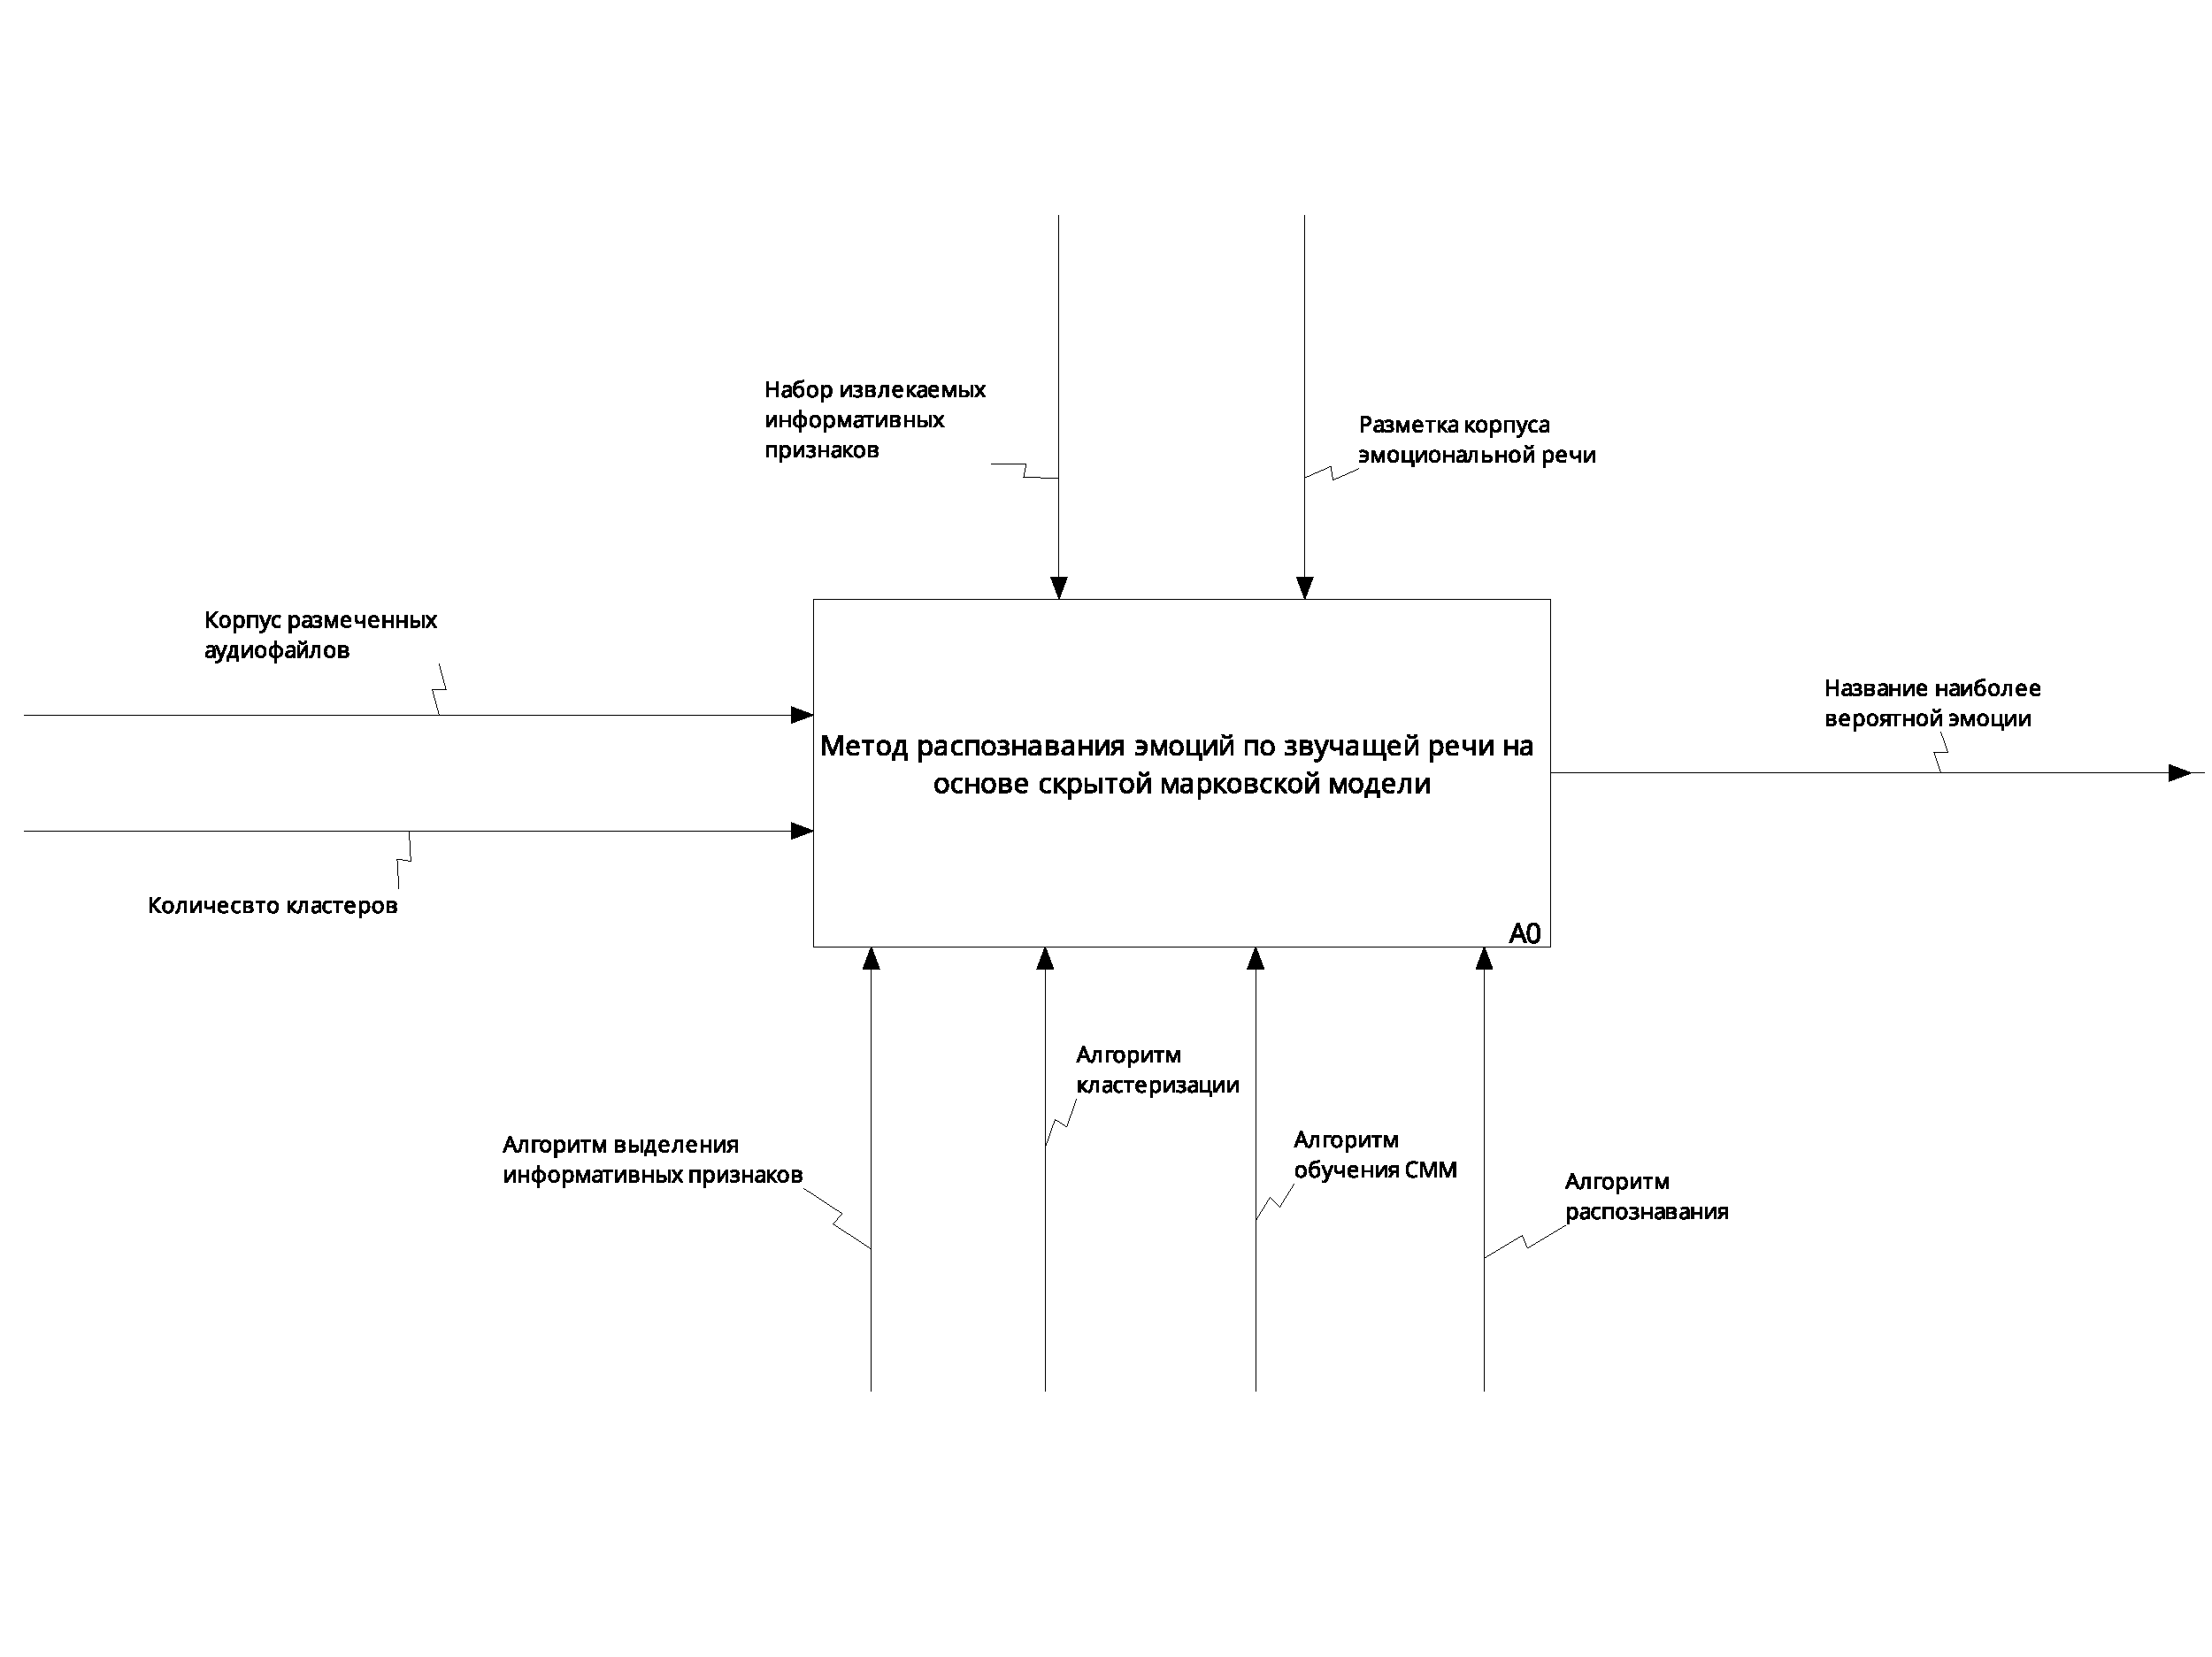
\includegraphics[width=\linewidth]{assets/01_A0}
	\caption{IDEF0-диаграмма нулевого уровня}
	\label{fig:idef0}
\end{figure}
Корпус данных должен быть подготовлен к использованию классификатором -- а именно, должно быть установлено однозначное соответствие аудиофайл-эмоция согласно представленной в наборе разметке. Под исследуемую задачу по разметке и по языку подходят следующие наборы: RUSLANA и DUSHA. Однако, корпуса RUSLANA на данный момент нет в открытом доступе.

Из аудиозаписей должны быть выделены информативные признаки. Поскольку сигнал должен быть разбит на кадры (фреймы) небольшой длительности, использование просодических признаков не имеет смысла, следовательно, будут использованы спектральные признаки речевого сигнала. В качестве спектральных признаков, извлекаемых из аудиофайлов, было решено использовать мел-кепстральные коэффициенты, поскольку:
\begin{itemize}
	\item мел-кепстральные коэффициенты представляют собой широкий спектр признаков, которые могут быть маркерами конкретной эмоции, таких как громкость, длительность, скорость и ритм;
	\item мел-кепстральные коэффициенты более устойчивы к шуму, чем, например, частоты первых 4-х формант или джиттер, поскольку они учитывают особенности восприятия звуковой информации человеческим ухом.
\end{itemize}

Для обучения классификатора эти признаки должны быть поделены на кластеры. Обученный классификатор используется для распознавания эмоций.
%Из аудиозаписей должны быть выделены информативные признаки. Для обучения классификатора эти признаки должны быть поделены на кластеры. Обученный классификатор используется для распознавания эмоций.
